\documentclass[a4paper]{article}
\usepackage[utf8]{inputenc}
\usepackage{amsmath}
\usepackage{amssymb}
\usepackage{mathtools}
\usepackage{amsfonts}
\usepackage{lastpage}
\usepackage{tikz}
\usepackage{float}
\usepackage{textcomp}
\usetikzlibrary{patterns}
\usepackage{pdfpages}
\usepackage{gauss}
\usepackage{fancyvrb}
\usepackage[table]{colortbl}
\usepackage{fancyhdr}
\usepackage{graphicx}
\usepackage[margin=2.5 cm]{geometry}

\definecolor{listinggray}{gray}{0.9}
\usepackage{listings}
\lstset{
	language=,
	literate=
		{æ}{{\ae}}1
		{ø}{{\o}}1
		{å}{{\aa}}1
		{Æ}{{\AE}}1
		{Ø}{{\O}}1
		{Å}{{\AA}}1,
	backgroundcolor=\color{listinggray},
	tabsize=3,
	rulecolor=,
	basicstyle=\scriptsize,
	upquote=true,
	aboveskip={0.2\baselineskip},
	columns=fixed,
	showstringspaces=false,
	extendedchars=true,
	breaklines=true,
	prebreak =\raisebox{0ex}[0ex][0ex]{\ensuremath{\hookleftarrow}},
	frame=single,
	showtabs=false,
	showspaces=false,
	showlines=true,
	showstringspaces=false,
	identifierstyle=\ttfamily,
	keywordstyle=\color[rgb]{0,0,1},
	commentstyle=\color[rgb]{0.133,0.545,0.133},
	stringstyle=\color[rgb]{0.627,0.126,0.941},
  moredelim=**[is][\color{blue}]{@}{@},
}

\lstdefinestyle{base}{
  emptylines=1,
  breaklines=true,
  basicstyle=\ttfamily\color{black},
}

\pagestyle{fancy}
\DeclarePairedDelimiter{\ceil}{\lceil}{\rceil}
\def\checkmark{\tikz\fill[scale=0.4](0,.35) -- (.25,0) -- (1,.7) -- (.25,.15) -- cycle;}
\newcommand*\circled[1]{\tikz[baseline=(char.base)]{
            \node[shape=circle,draw,inner sep=2pt] (char) {#1};}}
\newcommand*\squared[1]{%
  \tikz[baseline=(R.base)]\node[draw,rectangle,inner sep=0.5pt](R) {#1};\!}
\newcommand{\comment}[1]{%
  \text{\phantom{(#1)}} \tag{#1}}
\def\el{[\![}
\def\er{]\!]}
\def\dpip{|\!|}
\def\MeanN{\frac{1}{N}\sum^N_{n=1}}
\cfoot{Page \thepage\ of \pageref{LastPage}}
\DeclareGraphicsExtensions{.pdf,.png,.jpg}
\author{Nikolaj Dybdahl Rathcke (rfq695)}
\title{Advanced Computer Systems \\ Exam 2016}
\lhead{Advanced Computer Systems}
\rhead{Exam 2016}

\begin{document}
\maketitle

\section{Data Processing}
\subsection{}
If we sort the file by \texttt{time} (in $\mathcal{O}(n\lg n)$ time), we can find the $K$ closest events for each \texttt{eventid} in $\mathcal{O}(Kn)$ time - for a total of $\mathcal{O}(n\lg n + Kn)$ time. Note that we would have to sort by eventid in the end to mirror the output from the exam text, but this does not add anything to the complexity of the algorithm. However, since we cannot fit the entire click table in memory, we would need to use \textit{external sorting}, which typically works by sorting in chunks (at most $\sqrt{size(clicks)}$ chunks), writing them back to disk, and then using a merge strategy to sort the entire click table. External sorting can be done in $\mathcal{O}(n\lg n)$ though there is an I/O cost with it. The I/O cost can be reduced by using several disks for parallel reads and writes. We should not have any I/O cost associated with the location of the $K$ nearest events as we can assume $K$ is small and we only need to look at $2K$ events to find them. \\
This should be more effective than a naive search through the entire click table for each \texttt{eventid} which would have a complexity of $\mathcal{O}(Kn^2)$. This could be faster if it could be done entirely in memory, but since we cannot store all the output either, we would need a streaming algorithm for writing to disk as well. \\
The algorithm is correct as we sort by \texttt{time} and then for each \texttt{eventid} we look at the $K$ closest events. Since the closest events can be in both directions in the sorted table, we will have to check at most $2K$ events in the click table. Since we can discard the constant this yields the $\mathcal{O}(Kn)$ complexity term. To clarify, we can find the $K$ elements in $\mathcal{O}(K)$ time using the \textit{selection algorithm} to find the $K$'th closest event and then iterating through the same list to add the events that are closer. \\
The correctness of this algorithm is easily verified as we only look at the closest events in time and we make sure to check in both directions to ensure we get the $K$ closest events.

\subsection{}
We say it is one I/O cost when we perform a read or a write of a page from disk. The first sort (on \texttt{time}) will have to read all pages once from disk and write all pages once to disk in the step when we sort in chunks. This results in an I/O cost of $2P$. The merge step will have an I/O cost of $2P\lg P$, so that adds an I/O cost of $2P+2P\lg P$ for sorting the original click table. \\
When we find the $K$ nearest event, we need to read all pages again, so this adds a cost of $P$, but since we make new entries in the table, the table grows by a factor of $K$. So when we write back to disk, we actually have a cost of $KP$. This adds a cost of $P+KP$. \\
The last sort (on \texttt{eventid}) is the same as the first, but the table now has $KP$ number of pages, so this step adds a cost of $2KP+2KP\lg KP$. \\
Adding all this up gives us a total I/O cost of $3P+2P\lg P+3KP+2KP\lg KP + c$, where $c$ is some constant to represent the overhead we have when we sort or when we find the $K$ nearest events. We can use big O notation to write $\mathcal{O}(P\lg P+KP\lg KP)=\mathcal{O}(KP\lg( KP))$. We can make the reduction in the big O notation if we can expect $K\geq 1$ in which case that term dominates the other.

\section{Concurrency Control}
In the following questions, we use the notation $R(X)$ for reading an object $X$ and $W(X)$ for writing to an object $X$.

\subsection{a}
Consider the schedule:
\begin{verbatim}
  T1:      R(Y) W(X)
  T2: W(Y)           W(X)
  T3:                     W(X)
\end{verbatim}
This is view-serializable as the writes to $X$ from $T1$ and $T2$ does not matter, as it is overwritten by $T3$. We only need $T2$ to precede $T1$, so that $T1$ reads the right object $Y$. \\
However, it is not conflict-serializable as $T2$ needs to precede $T1$ due to object $Y$, but $T1$ also needs to precede $T2$, as the write to object $X$ should happen first for $T1$. In reality, this does not matter as no other transaction will read object $X$, since $T3$ overwrites it.

\subsection{b}
Consider the simple schedule:
\begin{verbatim}
  T1:      R(X)
  T2: W(X)      R(X)
\end{verbatim}
Which is conflict-serializable as $T2$ needs to precede $T1$ since it writes to object $X$ before $T1$ should read it, but $T1$ does not need to precede $T2$. \\
It cannot be generated by $2PL$, as $T1$ is not able to get a shared lock on object $X$ as $T2$ has an exclusive lock, which it will first release after its own read of object $X$.

\subsection{c}
Consider the schedule:
\begin{verbatim}
  T1:      R(X)
  T2: W(X)      R(Y)
\end{verbatim}
Which can be generated by $2PL$ as $T2$ would acquire an exclusive lock on $X$ and release it afterwards. Now, $T1$ will acquire a shared lock on $X$ and release it and $T2$ would acquire a shared lock on $Y$ and release it. This does not generate any conflicts. \\
It cannot be generated by strict $2PL$, as a transaction would release all its locks after it has performed all its operations. Therefore, $T2$ would acquire a lock on $X$ and $T1$ would not be able to acquire the lock on $X$ before $T2$ had finished.

\subsection{d}
Consider the simple schedule:
\begin{verbatim}
  T1:      R(Y)
  T2: W(X)      W(Y)
\end{verbatim}
This can be generated by strict $2PL$ as $T2$ would acquire an exclusive lock on $X$, $T1$ would then acquire a shared lock on $Y$ and release it and finally $T2$ would acquire an exclusive lock on $Y$ and release both locks. This does not produce any conflicts. \\
It cannot be generated by conservative strict $2PL$ as $T2$ would acquire exclusive locks on both $X$ and $Y$, which means $T1$ cannot get a shared lock on $Y$ before $T2$ finishes.

\section{Programming Task}
The implementation follows the same structure as the project we have worked on during the course, \texttt{acertainbookstore}. In the submitted code, all tests are set to local as default.

\section{Questions Regarding the Implementation}

\subsection{High-Level Design Decisions, Modularity, Fault-Tolerance}
The implementation strategy is very similar to that of \texttt{acertainbookstore} which we have been working on during the course from which I have reused some of the code. The methods implementing the \texttt{AuctionMarket} interface is found in the class \texttt{ConcurrentCertainMarket} in which we use locking to ensure before-or-after atomicity (discussed later). The class uses two maps, namely the \texttt{itemMap} and the \texttt{bidMap}, both of which uses an \texttt{itemID} as a key and the item or bid as values. These keep track of what items are up for sale and what bids have been made. When an epoch is finished, a call to \texttt{switchEpoch} is made which outputs an XML file with items and bids that have been matched. The matches have type \texttt{itemInfo} which is simply the info about both bid and item. The four methods throws exceptions when appropriate and are exposed as RPC's. Note there is only one interface and proxy, though in reality we might have one for admin clients as well - for methods such as \texttt{switchEpoch}. \\
The implemented RPC semantics is at-most-once semantics. The method \texttt{SendAndRecv} in the class \texttt{AuctionmarketUtility} sends a request and is blocking while it waits for a response. Two things can happen. Either there is a response or an exception is thrown. An exception can be a timed out exception, an unknown client exception or something similar. This is preferable as we do not want duplicate requests if the service is slow to provide a response for some reason. \\
The implementation satisfies all-or-nothing atomicity as all possible errors that can occur are checked before accessing the \texttt{itemMap} and \texttt{bidMap}. That is, if there is an error in a single item or bid in the set, it will throw the appropriate error and do nothing. The methods \texttt{queryItems} and \texttt{switchEpoch} satisfies all-or-nothing atomicity as no errors can occur assuming nothing has gone wrong when adding the items or bids. \\
The checkpointing of the final matching state after \texttt{switchEpoch} has been invoked is not sufficient for durability of all other operation in the auction market. The durability property ensures that once a transaction has been committed, it will stay committed even though there is a crash of some kind. The transactions are not in stable storage before the call to \texttt{switchEpoch}, so they can be lost in the meantime. To ensure a transaction is not lost, we would have to write it to stable storage right after the transaction has committed.

\subsection{Before-or-After Atomicity}
To make sure the operations satisfies before-or-after atomicity, the implementation uses locking. In particular, the implemented locking is conservative strict $2PL$ locking. So an operation requires all locks needed to do the operation, and will release all of them when all the work has been done. A lock for each of the maps, i.e. \texttt{itemMap} and \texttt{bidMap}, was used. \\
Since we are using conservative strict $2PL$, it means before-or-after atomicity is ensured. \\
We can guarantee consistency for read operations as we use exclusive and shared locks, which means we can not have a write action when we are already doing a read action. The locks, as mentioned, works on the entire maps, which means we do not need to worry about predicate reads. \\
Using conservative strict $2PL$ locking is simpler to implement and it is easier to guarantee correctness. But despite gaining a bit of concurrency from using exclusive/shared locks instead of just a single one, other $2PL$ variants provide even more concurrency as locks are either released earlier or acquired later. We also lock on the entire \texttt{itemMap} and \texttt{bidMap} where we could lock on single items instead. But the decision to use conservative strict $2PL$ locking was to make it easier to vouch for the correctness of the auction market.

\subsection{Testing}
To test the implementation, tests were made in three different categories. There are tests for correctness, tests for all-or-nothing atomicity and tests for before-or-after atomicity. \\
The tests for correctness are simple tests for the behavior of bids, i.e. that the final matching happens correctly. We do not need to test that an operation fails correctly, as this is what is done to test all-or-nothing atomicity. All possible errors that can be made for an operation has been tested. In each case, another valid item or bid is included in the operation. This way, we can verify that no changes has been made to the \texttt{itemMap} or \texttt{bidMap}, even though one item or bid could have been added. There are also tests for when all items or bids are valid, where it is verified they are all added. \\
To test the before-or-after atomicity, a test that uses two clients was constructed. One of the client continuously call \texttt{addItems} with $5$ new items. The other client keeps calling \texttt{queryItems} and checks if the returned number of items is equal to $0$ modulo $5$. If it is not, it means that the operation interfered with the \texttt{addItems} operation from the other client as it was not finished adding items. To verify the \texttt{bid} operation, you could design a test that uses two clients who both tries to add a bid with the same buyer on the same item. If there are two of the same bids (buyer ID and item ID is the same), it means they do not respect before-or-nothing atomicity. However, this would require that I exposed the \texttt{bidMap} to verify that there was only one bid, since the checkpoint from \texttt{switchEpoch} will only have one bid per item. But since we are using conservative strict $2PL$ and a bid overwrites (we test this under tests for correctness), we can argue that the operation does satisfy before-or-after atomicity assuming the locking has been implemented correctly. The \texttt{switchEpoch} operation was not tested for this, but again, if we can assume the locking is implemented correctly (that we get exclusive locks on both maps), it should satisfy before-or-after atomicity. \\
Note that all tests are successful (the before-or-after atomicity test takes a while to finish) both when they are local tests and when they are not.

\subsection{Experiments}
The experiment is designed in a way so that when we increase the number of threads, we also increase the number of all kinds of operations. That is, we do not have a constant number of seller threads. Instead, each operation has a percentage of happening, which is $20\%$ for \texttt{addItems} and \texttt{bid} and $60\%$ for \texttt{queryItems}. This is to simulate a realistic auction market. The experiment collected data for $2,4,..,20$ threads ($10$ datapoints) for both local and nonlocal tests. The experiment was run $4$ times for the non-local test and $10$ times for the local test as the results varied quite a bit more. Whenever a worker is spawned, it does 100 warm-up runs before doing 500 actual runs. For each number of thread, we get the throughput per nanosecond. Since this was done multiple times. the mean was taken and were used to produce Figure \ref{fig}. The experiment works with an initially empty auction market. These numbers were used, as more warm-up and actual runs made for painful benchmarking and they were sufficient to give an accurate indication of the throughput. The number of threads is also sufficient to illustrate the trends between threads and throughput. \\
The hardware used in the experiment is a dual-core (4-CPU) Intel(R) Core(TM) i5-2520M CPU @ 2.50GHz with 16GB of RAM. A good guess for how many threads produce the maximal throughput is the number of cores. This means we can expect it to peak around $8$ threads.
\begin{figure}[H]
  \centering
  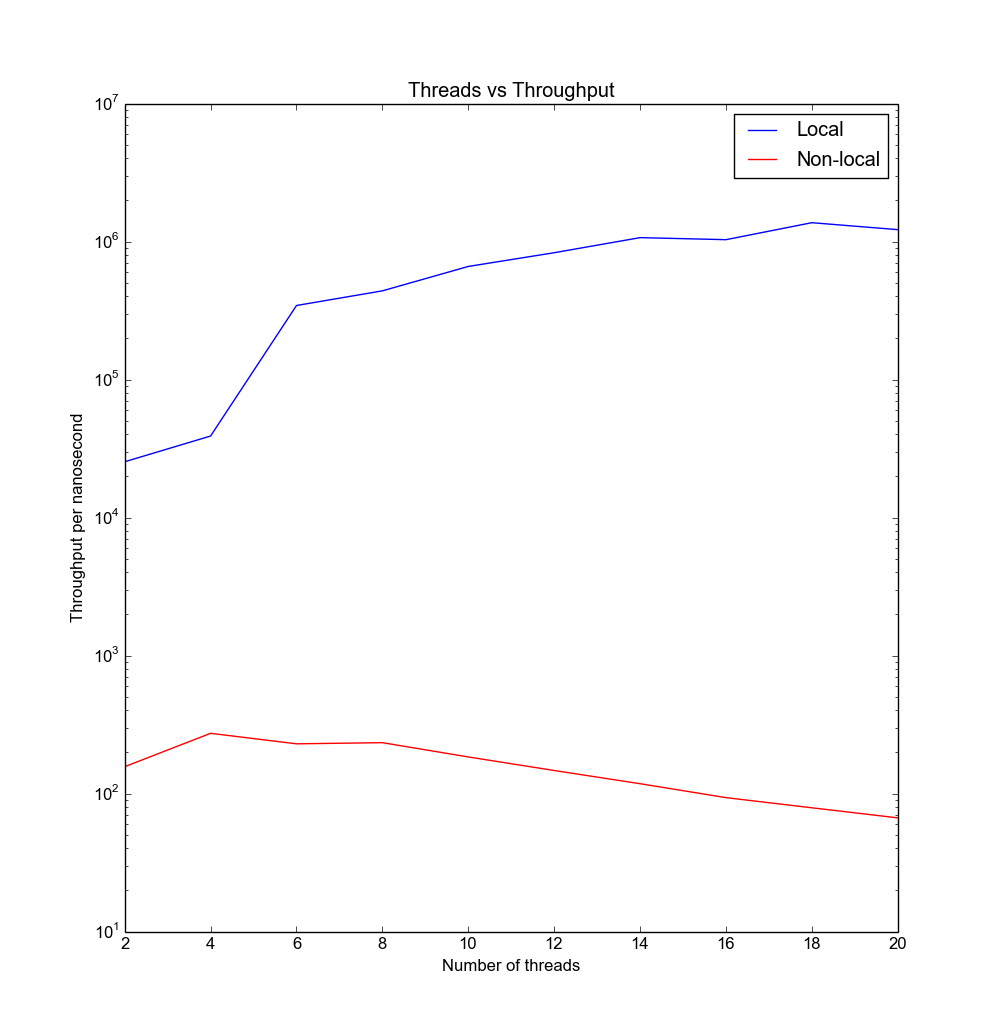
\includegraphics[scale=0.6]{fig1}
  \caption{Figure showing the relation between number of threads doing operations in the auction market and the throughput in nanoseconds.}
  \label{fig}
\end{figure}
$ $ \\
We have a lot more throughput in the local test, but it seems to even out very quickly as well. This is as we would expect, since increasing the number of threads surely will increase throughput, but at some point we have essentially gotten a maximum throughput and adding more threads will only make it worse. The throughput for the non-local test also behaves as we would expect. It increases in the beginning and the steadily falls as we get more and more threads as we would get a "queue" at some point when there are enough threads.

\end{document}
